% $Id$

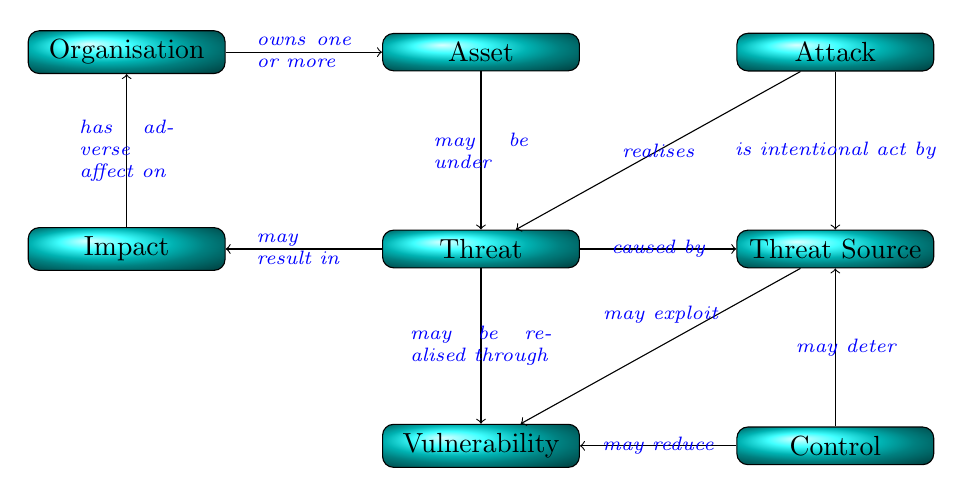
\begin{tikzpicture}
  \tikzstyle{term}=[minimum width=25mm,rounded corners,draw,ball color=cyan]
  \tikzstyle{lab}=[rounded corners,font=\scriptsize\itshape,text=blue]

  \node [term] (asset) at (4.5,5) {Asset} ;
  \node [term] (org) at (0,5) {Organisation} ;
  \node [term] (threat) at (4.5,2.5) {Threat} ;
  \node [term] (impact) at (0,2.5) {Impact} ;
  \path [->,draw] (org) edge node[lab] {\parbox{12mm}{owns one or more}} (asset) ;
  \path [->,draw] (asset) edge node[lab] {\parbox{12mm}{may be under}} (threat) ;
  \path [->,draw] (threat) edge node[lab] {\parbox{12mm}{may result in}} (impact) ;
  \path [->,draw] (impact) edge node[lab] {\parbox{12mm}{has adverse affect on}} (org) ;
  
  \node [term] (thsrc) at (9,2.5) {Threat Source} ;
  \path [->,draw] (threat) 
    edge node[lab] {caused by} (thsrc) ;

  \tikzstyle{second}=[ball color=cyan]
  \tikzstyle{third}=[ball color=cyan]

\onslide*<2>{\tikzstyle{second}=[ball color=red]}
\onslide*<3>{\tikzstyle{third}=[ball color=red]}
\onslide*<4>{\tikzstyle{third}=[ball color=yellow]}
\onslide+<2->{
  \node [term] (vul) at (4.5,0) {Vulnerability} ;
  \node [term] (control) at (9,0) {Control} ;
  \path [->,draw] (threat) 
    edge node[lab] {\parbox{18mm}{may be realised through}} (vul) ;
  \path [->,draw] (control) edge node[lab] {may reduce} (vul) ;
  \path [->,draw] (control) edge node[lab,xshift=4mm]
     {\parbox{18mm}{may deter}} (thsrc) ;
  \path [->,draw] (thsrc) edge node[lab,yshift=4mm] {may exploit} (vul) ;
}
\onslide+<3->{
  \node [term] (atk) at (9,5) {Attack} ;
  \path [->,draw] (atk) edge node[lab] {is intentional act by} (thsrc) ;
  \path [->,draw] (atk) edge node[lab] {realises} (threat) ;
}
\end{tikzpicture}
